\documentclass[output=paper,colorlinks,citecolor=brown]{langscibook}
\ChapterDOI{10.5281/zenodo.6393738}

\title{Learning Swahili morphology}

\author{John Goldsmith\affiliation{University of Chicago} and Fidèle Mpiranya\affiliation{University of Chicago}}

\abstract{We describe the results of automatic morphological analysis of a large corpus of Swahili text, the Helsinki corpus,
using Linguistica, an unsupervised learner of morphology. The result is a fine-grained analysis,
with some results corresponding to the familiar linguistic analysis, and  with others that are possible
only with exact quantitative measures available with computational analysis. The prefixal inflectional
morphology is largely done well, while the suffixal morphology is successfully analyzed in some cases and not
in others.}
\IfFileExists{../localcommands.tex}{
  \addbibresource{localbibliography.bib}
  \usepackage{langsci-optional,langsci-branding}
\usepackage{langsci-gb4e}
% \usepackage{langsci-textipa}
% \usepackage{langsci-glyphs}
\usepackage[linguistics]{forest}
\usepackage{tabto}
\usepackage{multirow}
\usepackage{bbding}

\usepackage[normalem]{ulem}

\usepackage{tikz-qtree}

\usepackage{enumitem}

\usepackage{multicol}
\usepackage{stmaryrd} %double brackets

\makeatletter
\let\pgfmathModX=\pgfmathMod@
\usepackage{pgfplots,pgfplotstable}%
\let\pgfmathMod@=\pgfmathModX
\makeatother
\usepgfplotslibrary{colorbrewer}
\usetikzlibrary{fit}

\usepackage{jambox}
\usepackage{tikz-qtree-compat}
\usetikzlibrary{arrows, arrows.meta}
\usepackage{longtable}
\usepackage{subcaption}

  \makeatletter
\let\thetitle\@title
\let\theauthor\@author
\makeatother

\newcommand{\togglepaper}[1][0]{
%   \bibliography{../localbibliography}
  \papernote{\scriptsize\normalfont
    \theauthor.
    \thetitle.
    To appear in:
    Change Volume Editor \& in localcommands.tex
    Change volume title in localcommands.tex
    Berlin: Language Science Press. [preliminary page numbering]
  }
  \pagenumbering{roman}
  \setcounter{chapter}{#1}
  \addtocounter{chapter}{-1}
}

\newcommand{\bari}{\ipabar{\i}{.5ex}{1.1}{}{}}
\newcommand{\notipa}[1]{\textnormal{#1}}

\newcommand{\agre}{\textsc{agr}-\ol{eene}}

\renewcommand{\emph}[1]{\textit{#1}} % resetting a setting from ling-macros-modified (I think?)

% forest settings to make compact but (mostly) straight-spined trees:
\forestset{
fairly nice empty nodes/.style={
            delay={where content={}{shape=coordinate,for parent={
                  for children={anchor=north}}}{}}
, angled/.style={content/.expanded={$<$\forestov{content}$>$}}
}}

\forestset{sn edges/.style={for tree={parent anchor=south, child anchor=north}}}

\newcommand{\bex}{\begin{exe}}
\newcommand{\fex}{\end{exe}}

\newcommand{\bxl}{\begin{exe}}
\newcommand{\fxl}{\end{exe}}

\newcommand{\ix}[1]{\textsubscript{#1}}
\newcommand{\alert}[1]{\textbf{#1}}
\newcommand{\ol}[1]{\textit{#1}}


			\usetikzlibrary{shapes,arrows,positioning,decorations,decorations.pathmorphing,intersections}
\forestset{
nice empty nodes/.style={
    for tree={calign=fixed edge angles},
    delay={where content={}{shape=coordinate,for siblings={anchor=north}}{}}
},
}

\definecolor{dark-gray}{gray}{0.3}

%\usepackage{dingbat,pifont}


%%%%%%%%%%%%For arrows%%%%%%%%%%%%%

\newcommand\Tikzmark[2]{%
  \tikz[remember picture]\node[inner sep=0pt,outer sep=0pt] (#1) {#2};%
}
\NewDocumentCommand\DrawArrow{O{}mmmmO{3}}{
\tikz[remember picture,overlay]
  \draw[->,line width=0.8pt,shorten >= 2pt,shorten <= 2pt,#1]
    (#2) -- ++(0,-#6\ht\strutbox) coordinate (aux) -- node[#4] {#5} (#3|-aux) -- (#3);
}
\NewDocumentCommand\DrawDotted{O{}mmmmO{3}}{
\tikz[remember picture,overlay]
  \draw[->,line width=0.9pt,dotted,shorten >= 2pt,shorten <= 2pt,#1]
    (#2) -- ++(0,-#6\ht\strutbox) coordinate (aux) -- node[#4] {#5} (#3|-aux) -- (#3);
}
\NewDocumentCommand\DrawLine{O{}mmmmO{3}}{
\tikz[remember picture,overlay]
  \draw[line width=0.8pt,shorten >= 2pt,shorten <= 2pt,#1]
    (#2) -- ++(0,-#6\ht\strutbox) coordinate (aux) -- node[#4] {#5} (#3|-aux) -- (#3);
}
%%%%%%%%%%%%%%%%%%%%%%%%%%%%%%%%%%%%%


\newcommand{\baru}{ʉ}
\newcommand{\baruH}{\'\baru}
\newcommand{\baruL}{\`\baru}

\newcommand{\ep}{ε}
\newcommand{\epH}{\'\ep}
\newcommand{\epL}{\`\ep}

\newcommand{\schwa}{ə}
\newcommand{\schwaH}{\'ə}
\newcommand{\schwaL}{\`ə}

\newcommand{\oo}{ɔ}
\newcommand{\ooH}{\'\oo}
\newcommand{\ooL}{\`\oo}

\newcommand{\ds}{\textsuperscript{
	\hspace*{-2pt}\begin{tikzpicture}
		\draw[-{>[scale=0.5]}] (0,0.4) --(0,0.25);
	\end{tikzpicture}}}

\newcommand{\ch}{t͡ʃ}
\newcommand{\dz}{d͡ʒ}

\newcommand{\tgl}{ʔ}

%shortcuts for the complementizers
\newcommand{\mbuL}{mb\baruL}
\newcommand{\mbuHL}{mb\baruH\baruL}
\newcommand{\mbuLH}{mb\baruL\baruH}
\newcommand{\la}{lá}
\newcommand{\nda}{ndà}

\newcommand{\tsc}[1]{\textsc{#1}}
\renewcommand{\textscb}{ʙ}
\newcommand{\ipa}[1]{#1} %disable IPA

\newcommand{\SM}[1]{#1}

\DeclareNewSectionCommand
  [
    counterwithin = chapter,
    afterskip = 2.3ex plus .2ex,
    beforeskip = -3.5ex plus -1ex minus -.2ex,
    indent = 0pt,
    font = \usekomafont{section},
    level = 1,
    tocindent = 1.5em,
    toclevel = 1,
    tocnumwidth = 2.3em,
    tocstyle = section,
    style = section
  ]
  {appendixsection}

\renewcommand*\theappendixsection{\Alph{appendixsection}}
\renewcommand*{\appendixsectionformat}
              {\appendixname~\theappendixsection\autodot\enskip}
\renewcommand*{\appendixsectionmarkformat}
              {\appendixname~\theappendixsection\autodot\enskip}

\renewcommand{\lsChapterFooterSize}{\footnotesize}
 
  %% hyphenation points for line breaks
%% Normally, automatic hyphenation in LaTeX is very good
%% If a word is mis-hyphenated, add it to this file
%%
%% add information to TeX file before \begin{document} with:
%% %% hyphenation points for line breaks
%% Normally, automatic hyphenation in LaTeX is very good
%% If a word is mis-hyphenated, add it to this file
%%
%% add information to TeX file before \begin{document} with:
%% %% hyphenation points for line breaks
%% Normally, automatic hyphenation in LaTeX is very good
%% If a word is mis-hyphenated, add it to this file
%%
%% add information to TeX file before \begin{document} with:
%% \include{localhyphenation}
\hyphenation{
affri-ca-te
affri-ca-tes 
Līk-pāk-páln
pro-sod-ic
phe-nom-e-non
Chi-che-wa
Lu-bu-ku-su
Ngbu-gu
Boyel-dieu
Mat-chi
pho-neme
Mil-em-be
Nyan-chera
Mc-Pher-son
Tsoo-tso
Sku-pin
dis-tin-guishes
con-ser-va-tion
Me-dum-ba
}

\hyphenation{
affri-ca-te
affri-ca-tes 
Līk-pāk-páln
pro-sod-ic
phe-nom-e-non
Chi-che-wa
Lu-bu-ku-su
Ngbu-gu
Boyel-dieu
Mat-chi
pho-neme
Mil-em-be
Nyan-chera
Mc-Pher-son
Tsoo-tso
Sku-pin
dis-tin-guishes
con-ser-va-tion
Me-dum-ba
}

\hyphenation{
affri-ca-te
affri-ca-tes 
Līk-pāk-páln
pro-sod-ic
phe-nom-e-non
Chi-che-wa
Lu-bu-ku-su
Ngbu-gu
Boyel-dieu
Mat-chi
pho-neme
Mil-em-be
Nyan-chera
Mc-Pher-son
Tsoo-tso
Sku-pin
dis-tin-guishes
con-ser-va-tion
Me-dum-ba
}
 
  \togglepaper[1]%%chapternumber
}{}

\begin{document}
\SetupAffiliations{mark style=none}
\maketitle 

\section{Introduction}\label{sec:goldsmith:1}

In this paper we would like to explain some of the things that we have learned from a project on the learning of morphology. ``Learning of morphology'' in this context means using an algorithm which takes a large amount of text from a language, and draws conclusions about what are the roots, affixes, and principles of word construction (from roots and affixes) in this particular language. The crucial fact to bear in mind is that the algorithm is to have no prior knowledge of the language that we give to it. Whether the language is English or is Swahili, the learning algorithm starts from the same point; any differences that it draws between the two derive entirely from the data, and not from anything that we have given to the algorithm. 

That sounds like a tall order, and in some ways it is. But we can offer the following as motivation for this work. When we teach an introductory course on linguistics, we always reserve the second class on morphology for an experiment. We begin by putting a word on the board: \textit{ninasema}, but we do not tell them this is from Swahili. We ask if anyone knows what it means or what language it comes from; if someone does know, we tell them to be quiet for the rest of the class. Then we ask everyone else to divide it into morphemes. There is silence, of course, because the students think they have no idea what the right answer is. Then we ask them to guess how many morphemes there are here: one? two? more? Students guess there are at least two morphemes, and if pressed, typically offer a cut into \textit{nina-sema.}

Then we write \textit{unasema}, and ask them if this allows them to change their minds. Everyone with an opinion opines that the correct cuts are \textit{ni-nasema} and \textit{u-nasema}. When we ask why they do not like \textit{nina-sema} and \textit{una-sema} -- which, after all, would allow them to keep the guess that they started out with, when they knew only \textit{ninasema} -- they do not know why, but they are pretty sure that \textit{ni/u}\,+\,\textit{nasema} is right.

Then we consider a third word, \textit{anasema}, and the students feel confirmed in their judgment after the second word, since they can easily extend their hypothesis to \textit{ni/u/a}\,+\,\textit{nasema}. Again, we ask them why they do not want to go for \textit{nina/una/ana}\,+\,\textit{sema}, and although they cannot say why exactly, they are pretty confident that this last hypothesis is not right, because it is missing something. 

The next word is \textit{ninaona}, and the students easily conclude that there is a break after \textit{nina} (comparing \textit{ninasema} and \textit{ninaona}) and furthermore, the word should be divided up as \textit{ni-na-ona}. The next two words we offer are \textit{ninampiga} and \textit{tunasema}. The first they break up as \textit{ni-na-mpiga}, and the second as \textit{tu-na-sema}. How about \textit{ninawapiga}? That must be \textit{ni-na-wa-piga}, and then they realize we must go back and reanalyze \textit{ninampiga} as \textit{ni-na-m-piga}. So far we have what we see in \figref{blind-analysis}.

The point to bear in mind is that the students have done this without being told what the Swahili words mean in English. At some point we explain that in other linguistics courses, the teacher gives their students the same words along with their English translations, but we tell them that we do not think it is necessary to know the meanings of the words to find the morphemes, and that the external form (which is to say, the spelling) is enough to discover the right morphological structure. By the end of the class, we have analyzed about 30 Swahili words, and found the right structure, at which point we tell them what the various morphemes mean in English, and briefly show the template of the Swahili verb, as in \figref{sketch1}. We have indicated tense markers with double and verbal roots with single underlining, respectively, for the reader's convenience, here and below. 



\begin{table}
\begin{tabular}{llll} \lsptoprule
ni & na & $\emptyset$ & sema \\
u &     & wa & ona \\
a &     & m  & piga \\ \lspbottomrule
\end{tabular}
\caption{Blind analysis}
\label{blind-analysis}
\end{table}

\begin{figure}
\begin{sideways}
\begin{tabular}{l}  
$ \left\{ \begin{tabular}{c} \textsc{subject}\\ \textsc{markers}  \\ ni \\ u \\a\\tu\\m\\wa\\\ldots  \end{tabular} \right\}  
\left\{ \begin{tabular}{c} \textsc{tense}\\\textsc{markers}\\\uline{na}\\\uline{li}\\ \uline{taka} \\ \uline{me}\\ \uline{ka}\\ \ldots  \end{tabular}  \right\} 
\left\{ \begin{tabular}{c} \textsc{object}\\\textsc{markers}\\ $\emptyset$ \\ni\\u\\m\\tu\\m\\ \ldots  \end{tabular}  \right\} 
\left\{ \begin{tabular}{c} \textsc{rel cl}\\\textsc{markers}\\ $\emptyset$ \\ye\\o\\cho\\vyo\\yo\\ \ldots  \end{tabular}  \right\} 
\left\{ \begin{tabular}{c} \textsc{stems}\\ \uuline{sem}  \\ \uuline{fany} \\\uuline{ingi}\\\uuline{tak}\\\uuline{to}\\\uuline{fuat}\\ \ldots  \end{tabular}  \right\} 
\left\{ \begin{tabular}{c} \textsc{extensions}\\an\\ish\\ik\\\ldots  \end{tabular}  \right\}$

$\left\{ \begin{tabular}{c} \textsc{final}\\ \textsc{vowel}\\a\\i\\e  \end{tabular}  \right\}$

\end{tabular}
\end{sideways}
\caption{Sketch of Swahili verb structure}
\label{sketch1}
\end{figure}
 
From this we draw the conclusion that it is possible to learn Swahili morphology even when you do not know another language to compare it to. This is a welcome conclusion, because this is a task that all Swahili-speaking children must undertake when they are two or three years old. 

But how exactly do the students do this? If we say they just use common sense, that is certainly true, but common sense is notoriously difficult to analyze. Furthermore, there is every reason to believe that this particular task is part of the language-learning capacity, so we have a very real professional interest in puzzling out exactly what this learning process is. It is for this reason that we began to develop an algorithm that learns the morphological structure of words, but with no access to meaning. In fact, we have developed several different approaches (and we are still looking for the best one), all of which we put under the umbrella name \textit{Linguistica} \citep{Goldsmith2001,Goldsmith2006,Goldsmith2010}.

How well can an automatic morphology analyzer deal with Swahili today? It has a long way to go before we can see it as comparable to a freshman taking a linguistics course using common sense. Still, there is a lot that it does right -- which is to say, there are a lot of linguistic generalizations that it does observe. While there are interesting and complex matters of morphophonology in Swahili (loss of a vowel before another vowel, \textit{ky} becoming \textit{ch}, etc.) we can approach the problem of morphology before solving problems of morphophonology. What Swahili offers is a large range of affixes of similar sizes, and it is quite a challenge for an algorithm to break down a word into morphemes.

The present paper offers an overview of how Linguistica analyzes Swahili words. Its value at this point is not that it does a better job of analysis than a human, but rather that it can do a careful study of the morphology of a text so that we can ourselves more easily discover what it is that we are looking at. Linguistica serves as a tool to let us better understand what the data are that we are looking at when we explore a language on a large scale.\largerpage

We believe that this work will be of interest to readers in different categories. For the linguist who knows Swahili, the results are interesting because such a linguist sees what can be learned in an explicit procedure of this sort. For such a linguist, Linguistica really serves as a microscope through which the details of the language emerge -- almost visually. For the linguist interested in morphology, the work is of interest for what it says about the linguistic analysis of morphemes. The central operation here is -- so to speak -- \textit{split}; the challenge for language learning is finding the pieces that the grammar of language organizes. One way to say this is that we are figuring out where a language-learner performs a ``split'' operation, turning an unanalyzed string into its component pieces. \textit{Split}, in this sense, is the flip-side to the process of \textit{Merge}, so much discussed in the current literature. \textit{Merge} makes sense only once we have developed the broad strokes of the rule of \textit{Split}!


\section{Earlier work in this area}

There was a good deal of work in computational morphology in general, and in automatic learning of morphology in a number of cases, during the last decade of the 20th century and the first decade of the present century, including significant work on Swahili and a number of other Bantu languages. Some of this was motivated by an interest in automatic learning of morphology (see the overviews in \citealt{Goldsmith2010} and \citealt{GoldsmithEtAl2017}), and much was motivated by practical goals. These goals included developing morphological analyzers that could be used in speech recognition systems and in machine translation, and also methods that could be used to parse very large Swahili corpora, such as the one developed as the Helsinki Corpus of Swahili, notably the SALAMA project described by \citet{Hurskainen1992, Hurskainen1999, Hurskainen2004Compilers}. 

\begin{sloppypar}
The SALAMA project developed the linguistic resources that made this work possible, notably the corpus of Swahili that contained over 300,000 distinct words. Without the resources that this project created, our work would not have been possible at all. 
\end{sloppypar}

\citet{DePauwDeSchryver2008} provide an overview of much of that work, and they discussed work on a number of languages, including Northern Sotho, Zulu, Xhosa, and Tswana (see also \citealt{DePauwEtAl2009}). There was a special issue on African Language Technology in \textit{Language Resources and Evaluation} in 2011 which provided coverage of work that was being done at that time.  As just noted, much of the work had practical goals in mind, such as improving speech recognition \citep{GelasEtAl2012} and machine translation systems, and in such a context, focusing on the development of a system that operates with no language-particular knowledge is a luxury item that has few rewards. Several researchers applied one of the Morfessor systems, such as \citet{GelasEtAl2012} and some applied one of the Linguistica systems.  \citet{Linden2008} explores predicting unseen Swahili words; see also \citet{Muhirwe2007}.

 
%COMMENTED BY AUTHORS De Pauw and de Schryver 2008. They describe a range of projects on Bantu languages, including work on Northern Sotho, Zulu, Xhosda Swazi and Tswana. Smaller projects on Shona, Ndebele, Kwanyama and Rwanda. Also Kimmo-style systems for Gusii and Swahili. SALAMA presented by Hurskainen 1992, 1996, 2004, used to parse the Helsinki Corpus of Swahili (HCS, Hurskainen 2004a).  Two web-based interfaces: Kamusi Project and the ONline Swahili-English Dictionary. 


Several efforts have included ``data-driven'' learning, including  \citet{DePauwEtAl2006} on Swahili, \citet{DeSchryverDePauw2007} on  Northern Sotho. Unsupervised learning is discussed for  Luo (Nilotic) in \citet{DePauw2010},  and for Gikuyu \citep{DePauwWagacha2007}. \citet{Linden2008} discusses semi-supervised lemmatization of Swahili.
   

\section{What is a morphological analysis?}

What is a morphological analysis? This question is not anodyne; our answer to it determines what we expect of our learning algorithm. In much of the work in this area over the last 20 years, the answer has been that a morphological analysis is a division of each word into the pieces called \textit{morphs}. We would like to accomplish more than that; we would like to discover more of the principles that determine the order and the distributional possibilities of roots and affixes.\footnote{The view that the study of words was the study of how the words are composed of morphs and morphemes was viewed by most American linguists of the first half of the 20th century as the greatest American contribution to linguistics, second only to the setting of the phoneme on a firm methodological basis.}  

We can learn an extremely important lesson by looking at what the students did as they examined the Swahili words and proposed an analysis, based purely on form. They became convinced that they had found the right pattern, one that really gets at something \textit{true} about the data,  when they discovered sets of morphemes that take the form in \figref{morphology} for English or Swahili. Of course, the patterns there hold not just for these two verb stems, but for a very large set of stems, and this is even more true in the case of Swahili.

\begin{figure}
  \[ \left\{ \begin{tabular}{c} jump \\ laugh  \end{tabular} \right\}  \left\{ \begin{tabular}{c} $\emptyset$ \\ed\\ing\\s \end{tabular}  \right\} \]

 \[ \left\{ 
\begin{tabular}{c} 
ni \\ u \\ a 
\end{tabular} 
\right\}
\left\{ 
\begin{tabular}{c}
\uline{na} 
\end{tabular}  
\right\}  
\left\{ 
\begin{tabular}{c} 
$\emptyset$ \\ wa  \\ m 
\end{tabular} 
\right\} 
\left\{ 
\begin{tabular}{c} 
\uuline{sem} \\ \uuline{on} \\ \uuline{pig}  
\end{tabular}  
\right\}
\left\{ 
\begin{tabular}{c}
a 
\end{tabular}  
\right\} 
\]
\caption{Two pieces of morphology}
\label{morphology}
\end{figure}
 


 

%\begin{minipage}{.4\textwidth}
\begin{table}
\begin{tabular}{*6{l}}\lsptoprule
class & verbal SM & nominal pr. & adjectival pr.  & \multicolumn{2}{l}{pronominal pr.} \\\midrule
\textsc{prs.1sg} & ni &  --  & m- \\
\textsc{prs.1pl} & tu & --  & wa- \\
\textsc{prs.2sg} & u & --  &m-  \\
\textsc{prs.2pl} & m & -- & wa- \\
1 & a & m, mw  & m, mw & yu & but w\slash -- V \\
2 & wa & wa & wa & wa & but w\slash -- V\\
3 & u & m, mw & m & u&  but w\slash -- V \\
4 & i & mi & mi & i& but y\slash -- V  \\
5 & li & ji/$\emptyset$ & ji/$\emptyset$ & li & but j\slash -- V  \\
6 & ya & ma & ma & ya & but y\slash -- V  \\
7 & ki &ki & ki & ki & but ch\slash -- V \\
8 & vi & vi & vi & vi & but vy\slash -- V  \\
9 & i & n/$\emptyset$ & n/$\emptyset$  & i & but y\slash -- V  \\
10 & zi & n/$\emptyset$ & n/$\emptyset$  & zi & but z\slash -- V    \\
11 & u & u  & m  \\
14 & u & u & m \\
15 & ku, kw & ku, kw  & ku, kw\\ 
16 & pa & pa\\
17 & ku & ku \\
18 & m & m \\
\lspbottomrule
\end{tabular}
\caption{Class-based prefixes\label{class-based-system}}
\end{table}
 
  
These representations show clearly how a good morphological analysis captures excess information that would be present if we were to simply list all of the relevant words. Morphological analysis starts with words, identifies redundancies, and uses those redundancies to create a representation in which what is stated is the essence of the grammatical description, that is, what makes the language what it is. In the present case, the word \textit{redundancy} means needless repetition of a string of phonemes (or letters).

So how can we devise an algorithm to accomplish this? As our linguistics students showed us, there is a great deal to be learned from comparing pairs of words, which is what they did as we gave them words, one at a time. Zellig Harris, in a famous paper \citep{Harris1955}, suggested that a good estimate of the likelihood of a morpheme break could be devised if we take an alphabetized list of words, and with each word, we trace through it one letter at a time, asking after $n$ letters, how many different letters  those first $n$ letters were followed by in our particular corpus from the language. For example, after \textit{jum}, two letters (\textit{p} and \textit{b}) were found in a corpus we were looking at recently (from \textit{jump} and \textit{jumble}), while after \textit{jump}, four letters followed (\textit{space}, \textit{e}, \textit{i}, and \textit{s}), and after \textit{jumpi} only one letter follows (\textit{n}).

Harris believed that by measuring this \textit{successor frequency} we could find good candidates for morpheme breaks, and he was right. But the strings that we discover in this way are only candidates; many of them are not at all morphemes, and many morphemes are not discovered by Harris's method (or rather, by his methods). We hesitate to show the reader what can go wrong; it may cause them to wonder why we are using these methods. Here is a summary of the first stage of the algorithm that Linguistica employs. If we are seeking suffixes:
\begin{enumerate}
\item  Find every position in each word where the successor frequency is 2 or greater, and imagine splitting the word there, with the piece on the left a potential stem, and the piece on the right the (potential) stem's \textit{continuation}. We say ``potential'' here, because this piece has more tests to pass before it can be called a stem.

\item  Having done that, for each potential stem $S$, gather together all of $S$'s continuations, and alphabetize them. (For example, the potential stem \textit{jump} might be linked to the set of suffixes $\emptyset$, \textit{ed, ing, s}.) 

\item   Consider all of these continuations, and find those which are exact matches as the continuation of two different potential stems. For example, \textit{walk} might also be linked to the set of suffixes in $\emptyset$, \textit{ed, ing, s}. If we find such pairs of \textit{multiple stems} and also \textit{multiple suffixes}, we call that a \textit{signature}.
\end{enumerate}

If we are seeking prefixes, we do much the same, except that we do it in the reverse direction. We scan each word from right to left, looking to see how many different letters \textit{precede} each string reaching to the end:

\begin{enumerate}
\item  Find every position in each word where the predecessor frequency is 2 or greater, and imagine splitting the word there, with the piece on the right a \textit{potential stem}, and the piece on the left the potential stem's continuation (in this case, however, the continuation is in a right-to-left direction, counter-intuitive as that may seem).

\item  Having done that, for each potential stem $S$, gather together all of $S$'s continuations, and alphabetize them. (For example, the potential stem \textit{-tabu} (`book' in Swahili) might be linked to the set of prefixes \textit{ki-, vi-} `\textsc{sg}, \textsc{pl}'.) 

\item  Consider all of these continuations, and find those which are exact matches as the continuation of two different potential stems. (For example, \textit{-tu} `thing' in Swahili might also be linked to the set of prefixes in \textit{ki,vi}.) If we find such pairs of \textit{multiple stems} and also \textit{multiple affixes}, we label that a \textit{signature}.  A small Swahili text might include the signature \{ki,vi : tabu,tu\}.
\end{enumerate}

 


This account assumes that we already know where the points are where the successor frequency (or predecessor frequency) is greater than 1, and it turns out that there is a simple way to find all those points, in all the words, and it requires much less work than one might imagine. First, alphabetize the list of words, and then go through that list looking only at pairs of words that are adjacent on the list (such as \textit{walked, walking}, for example). Scan the two words from left to right (if we are looking for suffixes) or right to left (if we are looking for prefixes), and stop at the first point where the two words differ by a letter. The algorithm takes what is to the left of that point as a potential stem, and it then moves on to the next pair of words. This process is both simple and fast, from a computational point of view.

It is not right to say that the algorithm is finding stems at this point. We will let it analyze Swahili to find prefixes, and in so doing, we are finding the left-most set of morphemes, and treating everything that follows as an unanalyzed whole, which we call for now simply a ``potential-stem.'' In fact, that potential-stem contains many morphemes within it; we are now engaged in simply slicing off the leftmost prefixes of the words in Swahili, and we have just called what follows a ``potential stem.''  We will continue to cut the potential-stem down to smaller morphs as that becomes possible. Thus in most of the cases we look at below, the ``potential'' stems that are computed are themselves analyzable into morphs (at a later stage in the computation, as well as in our heads). In order to avoid the ambiguity of the phrase ``potential stem,'' we will create a new term, \textit{parastem}, to refer to this. A signature is composed of a set of affixes and a set of parastems, and the parastems may themselves be analyzed further in additional signatures. A parastem that can be broken down no further is a stem.

As we observed at the beginning of this section, within the community of computational linguists working on the problem of automatic learning of morphology, different researchers have begun with different assumptions about what the task is. Some linguists have focused on the problem of segmentation, which means dividing a word up into successive morphs, while others (perhaps skeptical about the notion of morph or morpheme) seek to tag any given word with the morphosyntactic features that it bears. Our work falls in the former group -- that is, we are very concerned with finding the proper analysis of a word into consecutive morphs. In addition, we would like to provide an analysis of how morphemes relate to one another in a word. Traditionally, linguists have spoken about relationships in praesentia, relations between morphemes that appear in a given word, and relationships in absentia, which is to say, the way in which multiple morphemes are alternatives to one another in a particular position in a word's morphology. We are interested in learning as much as possible about this aspect of a language's morphology as well.
 

Our interest here is exploratory. We are not in a rush to develop a practical tool; we have the opportunity to take some time and look at what kind of evidence regarding linguistic structure can be found by looking carefully at language data.\footnote{The algorithm that we employ here has the following stages. We will describe the process of prefix discovery, and the mirror image of it is used for suffix discovery. First, we alphabetize the list of words from the right-end of each word, then we look at each pair of adjacent words on this list, and determine find the rightmost letter whereby the two words disagree. We take the material to the right of that point as a \textit{protostem}. For each word $w$ that ends with protostem $t$, we take $e$ to be $t$'s extension if $w=e+t$ (i.e., if $e$ is what precedes $t$ in word $w$). We call each set of extensions to a protostem a \textit{protosignature}. We collect all protosignatures that are associated with at least two protostems. We create a set of signatures which consist of a collection of extensions and all of the stems which occur with exactly those extensions in the corpus. If all of the stems in a signature end with the same letter or string of letters, that letter or string of letters is moved from the stems to the extensions. Two further functions are used to identify licit morphemes in the extensions in the system used here.}


\section{Morphology of the left edge of the Swahili verb}

We used the Helsinki corpus of Swahili, which has about 300,000 distinct words. When we applied the current Linguistica algorithm above to 300,000 words to find prefixal signatures, we found 3,434 signatures; when we added an entropy-based filter,\footnote{That filter is roughly this: when the algorithm makes a prefix cut, in light of what we have said so far, it is because as we scan from right to left, a spot is found where there are two alternative options: e.g., as we scan \textit{kitabu} and \textit{vitabu} from right to left, a break will be created before the common stem \textit{-itabu}, though this is in fact wrong. Indeed, throughout the corpus, when a signature \textit{k=v} would be uncovered, it will always be followed by exactly one phoneme option: the vowel \textit{i}. The location of true morpheme breaks always involves options both to the left and to the right (which is to say, both prior in time and forward in time). We measure this notion of \textit{options} by the entropy of the final letter right before and right after a proposed morpheme break, and if (as with \textit{k-itabu, v-itabu}) zero entropy is discovered (which is just a way of saying that only one letter is present), the algorithm proceeds to create other splits until a non-zero entropy is found. In the case of \textit{kitabu}, this means adding the break \textit{ki-tabu, vi-tabu}, which has a non-zero entropy after the break, since many different letters follow \textit{ki-} and \textit{vi-}, such as we see in \textit{kilima, vilima} `hill, hills'.}  1,235 signatures remained, and it is this set of signatures that we will describe.  

In some ways, using Linguistica is a bit like using a microscope, and just like when we use a microscope for the first time, it takes a bit of experimenting before the picture comes sharply into focus. Let us begin our tour, then, with a rough statement of the position of morphemes in finite Swahili verbs, and a summary of what Linguistica gleans from a large corpus. 

The textbook description of Swahili is much as given in \figref{sketch}, while Linguistica's conclusions for the left side and the right side of the Swahili verb are given in \tabref{table-iterations-prefix}. The first figure concerns the initial subject marker position, the following tense marker position, and the position after the tense marker. It does not properly distinguish object markers, such as the \textit{-ki-} in \textit{ni-li-ki-som-a} `I read it'  from the relative clause marker  \textit{cho} in \textit{ki-tabu ni-li-cho-ki-soma} `the book that I read'.     

  
\begin{figure} 
$\bigg[
\begin{tabular}{@{}c@{}} 
\textsc{subj}\\
\textsc{marker}\\
\end{tabular}
\bigg] 
\bigg[
\begin{tabular}{@{}c@{}} 
\textsc{tense}\\
\textsc{marker}\\
\end{tabular}
\bigg] 
\bigg[
\begin{tabular}{@{}c@{}} 
\textsc{rel cl}\\
\textsc{marker}\\
\end{tabular}
\bigg] 
\bigg[
\begin{tabular}{@{}c@{}} 
\textsc{object}\\
\textsc{marker}\\
\end{tabular}
\bigg] 
\bigg[
\begin{tabular}{@{}c@{}}
\textsc{verb}\\ 
\textsc{root}\\
\end{tabular}
\bigg] 
\bigg[
\begin{tabular}{@{}c@{}} 
\textsc{exten-}\\
\textsc{sions}
\end{tabular}
\bigg] 
\bigg[
\begin{tabular}{@{}c@{}} 
\textsc{final}\\
\textsc{vowel}
\end{tabular}
\bigg] 
$
\caption{Sketch of Swahili verb morphology}
\label{sketch}
\end{figure}



 \begin{figure}

%{\color[rgb]{0.000000,0.000000,0.000000}

\begin{tabular}{l}
$\left\{
\begin{tabular}{c} 
\textsc{subject}\\
\textsc{markers}\\
$\emptyset$  \\
a \\
i \\
li\\
m\\
ni\\
pa\\
tu\\
u\\
vi\\
wa\\
ya\\
zi \\ 
\ldots 
\end{tabular} 
\right\} 
$


$\left\{ \begin{tabular}{c} \textsc{tense}\\\textsc{markers}\\ \uline{
$\emptyset$}\\ 
 \uline{ka} \\
 \uline{ki} \\
 \uline{li}\\ 
\uline{lio}\\
 \uline{me}\\
 \uline{na} \\
  \uline{ta} \\
 \ldots  
\end{tabular}  
\right\} 
\left\{ 
\begin{tabular}{c} 
\textsc{rel clause}\\
\textsc{and object} \\ 
 \textsc{markers}\\ 
$\emptyset$\\
ji  \\
m\\
nge \\ 
ni\\ 
po\\
vyo \\ 
ta\\
wa  \\
zo \\ 
\ldots  
\end{tabular}
  \right\} 
\left\{ 
\begin{tabular}{c} 
\textsc{roots}\\ 
\uuline{sem}a  \\ 
\uuline{fany}a \\
\uuline{ingi}a\\
\uuline{tak}a\\
\uuline{to}a\\
\uuline{fuat}a\\ 
\ldots 
 \end{tabular}
  \right \}  
$
\end{tabular}
%\caption{\textsc{Summary of first three iterations of prefix discovery}}
\caption{Summary of Linguistica's analysis of the left half of the Swahili verb}
\label{table-iterations-prefix}
\end{figure}
   
 
Indepently of prefix discovery, Linguistica analyzes the right-end of the word, and the major part of its conclusions are summarized in  \figref{final-signatures}. 
 

\begin{figure}
\begin{minipage}{.33\textwidth}\centering
$ \left\{
\begin{tabular}{c}   
bish\\ esh  \\ ez \\ ili \\ ish \\iz \\ki \\li\\mi\\ng\\sh \\ ti\\ uk \\ uli \\ uz \end{tabular} \right\} $
$\left\{ 
\begin{tabular}{c}$\emptyset$ 
\\w\\ 
\end{tabular}
\right\}   \left\{a \right\}$
\end{minipage}\begin{minipage}{.33\textwidth}\centering
$ \left\{ \begin{tabular}{c}an\\ik\\ish\\iz\\uk\\ush\end{tabular} \right\} 
\left\{ \begin{tabular}{c}$\emptyset$ \\i\\ \end{tabular} \right\} 
\left\{a \right\}$
\end{minipage}\begin{minipage}{.33\textwidth}\centering
$ \left\{ \begin{tabular}{c} an\\ish\\sh\end{tabular} \right\}  
\left\{ \begin{tabular}{c}$\emptyset$ \\iw\\ \end{tabular} \right\}  
\left\{a \right\} $
\end{minipage}
\caption{Three signatures from Linguistica's analysis of the right half of the Swahili verb\label{final-signatures}}
\end{figure}



 
However, the template given in these two tables gives only a superficial summary of Linguistica's analysis. Let us consider what happens with each slice of the analysis.

 
There are 1,235 signatures that emerge from the first iteration of prefixal analysis. What do these signatures say? What can we learn from them? It is natural to sort them in some way so that the most interesting signatures will appear at the top of the list, and there are several ways of sorting that come to mind. We might, for example, sort the signatures by the number of stems they contain, or we might sort them by the number of affixes. Both present us with interesting material. From a linguist's point of view, sorting them by the number of affixes is by far the more interesting. \figref{lattice}, which is presented to the user by Linguistica, shows how we can arrange the signatures in a lattice, where signatures with the same number of affixes appear on the same row, and in which the signatures in each row are sorted by decreasing numbers of stems (though we have departed from that latter point a bit to make the figures easier to read here).\largerpage
 
\begin{figure}
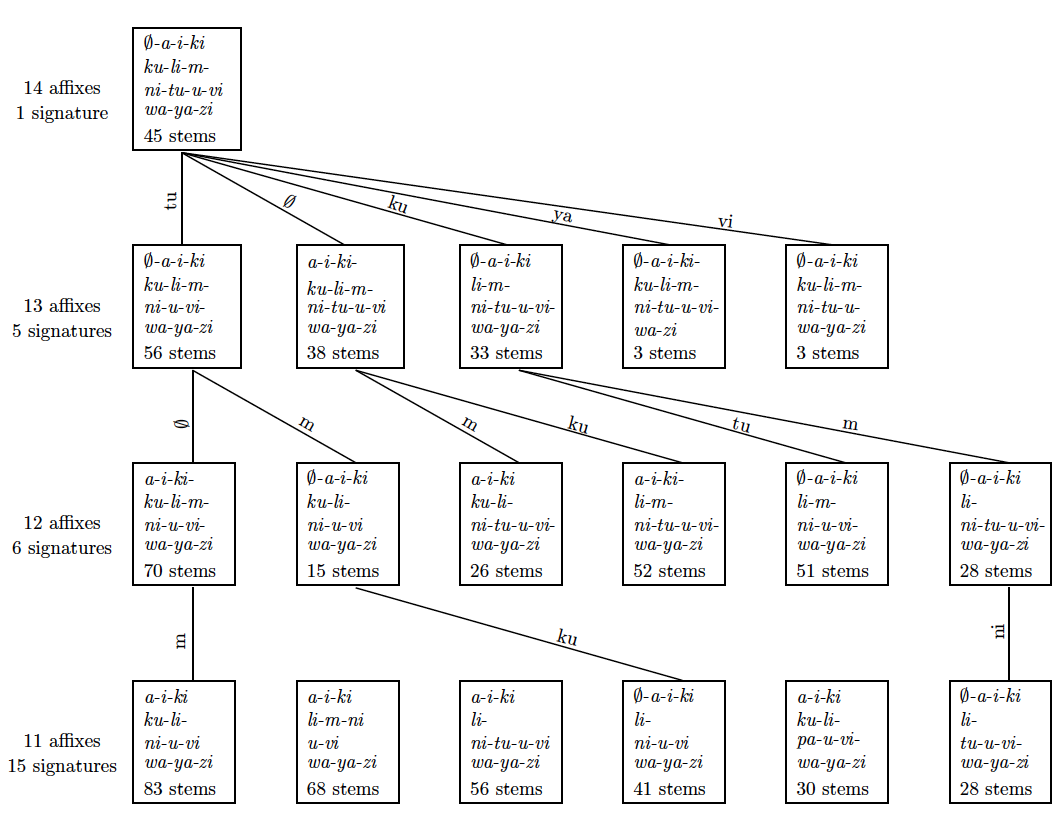
\includegraphics[width=\textwidth]{figures/top_of_lattice.png}
\caption{Top of the lattice of word-initial signatures}
\label{lattice}
\end{figure}

%===========================================================================%

\begin{table}  
\begin{tabular}{rr *{8}{r@{~~}}r} \lsptoprule
$N$ affixes  & $N$ signatures & \multicolumn{8}{l}{Stem counts in  individual signatures}\\\midrule
14 & 1 & 45  \\
13 & 5 & 56 & 38 & 33 & 3 & 3 \\
12 & 6 & 70 & 52 & 51 & 28 & 26 & 15   \\
11 & 15 & 83 & 68 & 56 & 41 & 30 & 28 & 16 & 11& 9 \ldots  \\
10 & 22 & 129 & 90 &  38 &  32 &  30 &  23 &  22 &  20 & 17    \ldots\\
9 &  34 & 205 &   46 &  32 &  29  &  20   &  19 &  16 &  16 & 15   \ldots\\
8 &   56 & 131 & 82 &  56 &  41 &  26 &  25 &  24 &  17 &  16       \ldots \\
\ldots \\
2 & 653 & 2419 &1297 & 1070 &  755 &  690 &  668 &  601 &  564 &  507    \ldots \\ \lspbottomrule
\end{tabular}
\caption{Word-initial signature counts}
\label{table2}
\end{table}

%%===========================================================================%
%
% 
\begin{sidewaystable}
\begin{tabular}{lllllllllllllllllll}\lsptoprule
Rank& Stem count & \multicolumn{15}{c}{Signatures} \\ \midrule
1 & 45 & ∅ & a &  i &  ki &  ku &  li &  m &  ni  &&  tu &  u &  vi &  wa &  ya &  zi \\
2 & 56 & ∅ & a &  i &  ki &  ku &  li &  m &  ni &   & &  u &  vi &  wa & ya  &  zi   \\
3 & 38 &      & a &  i &  ki &  ku &  li &  m &  ni  &&  tu &  u &  vi &  wa &  ya &  zi \\
4 & 33 &  ∅ & a &  i &  ki &  &  li &  m &  ni &   &  tu &  u &  vi &  wa &  ya &  zi  \\
5 & 3  & ∅ & a &  i &  ki &  ku &  li &  m &  ni &   &  tu &  u &  vi &  wa &    &  zi\\
6 & 3 & ∅ & a &  i &  ki &  ku &  li &  m &  ni &  &  tu &  u &   &  wa &  ya &  zi  \\
7 & 70 &    & a &  i &  ki &  ku &  li &  m &  ni  &&    &  u &  vi &  wa &  ya &  zi  \\
8 & 52 &   & a &  i &  ki &   &  li &  m &  ni &  &  tu  &  u &  vi &  wa &  ya &  zi  \\
9 & 51 & ∅ & a &  i &  ki &   &  li & m &  ni &   &   &  u &  vi &  wa &  ya &  zi\\
10 & 28  & ∅ & a &  i &  ki &   &  li &   & ni  &   &  tu &  u &  vi &  wa &  ya &  zi\\
11 & 26 & & a &  i &  ki & ku  &  li &    &  ni &   &  tu &  u &  vi &  wa &  ya &  zi \\
17 &  30 &  & a &  i &  ki &  ku &  li &   &    & pa &    &  u &  vi &  wa &  ya &  zi \\
719  & 191 && a &i &&&&&&&&u &&wa  \\  \lspbottomrule
\end{tabular}
\caption{Examples of word-initial signatures}
\label{topsigexamples}
\end{sidewaystable}


%%===========================================================================%

  


We need to explain carefully what the relation is between the several figures and tables given here. Each box in \figref{lattice} is a signature, and each corresponds to an individual \textit{row} in  \tabref{topsigexamples}. Each of these signatures corresponds to an individual \textit{number} that appears in the rightmost field of  \tabref{table2}, and the reader can see the correspondence by comparing the number which indicates the number of stems in each signature.

In \tabref{table2},  each line corresponds to a row in \figref{lattice} -- top row to top row, and then down from there. Each of the lines in the next table, \tabref{topsigexamples}, corresponds to \textit{one} of the individual signatures tallied in \figref{lattice} or \tabref{table2}. The first row in \tabref{topsigexamples} corresponds to the one signature with 14 affixes, and the five signatures in row 2 in \tabref{topsigstems} are the next five signatures in \tabref{table2} (or \figref{lattice}). 

\subsection{The top signature and its parastems}
The very top signature in \figref{lattice} is the largest signature, in that it has a  set of 14 prefixes: \textit{$\emptyset$-a-i-ki-ku-li-m-ni-tu-u-vi-wa-ya-zi} ; it does not contain the locative marker \textit{pa-}.\footnote{We consider the absence of \textit{pa} to be an error committed by Linguistica.} The vast majority of signatures beneath it are composed of subsets of those 14 prefixes. Each of the five signatures on the row for 13 affixes is missing one prefix from the one in row 14 (in both \tabref{table2} and \figref{lattice}), just as each of the signatures in row 12 is missing one from those above it, and these differences between the affixes comprising the signatures are marked on the lines in the figure. We have given 18 signatures in \figref{lattice} out of the total set of 1,235. 
 
Let us dig a little more deeply, and look at the parastems that are found in the top signatures (recall that a parastem is an element in a signature which may be analyzed in a later signature). Each parastem is sorted by, and listed with, its total occurrence count in the corpus in \tabref{topsigstems}. One does not see much that stands out with this frequency sorting, but we have sorted the stems alphabetically in \tabref{stems-alphabetized-1}. Here we have \textit{manually} underlined the tense markers and double-underlined the verb roots for the reader's benefit, and manually indicated morpheme breaks (these breaks have not been discovered by Linguistica yet). 
  
%===========================================================================% 
  
\begin{table}  

\begin{tabular}{*{3}{lr}} 
\lsptoprule 
na & 554,554 &          {rudi} & 1991 &          {li}{kubali}     & 564 \\ 
le & 33,130 &           {na}{hitaji} & 1783&     {na}{ingi}a    & 447 \\ 
ki{w}a & 20,663 &       {jadili} & 1514 &        {fik}e & 325 \\ 
pande & 10,230 &        {nge}ku{w}a & 1493 &     {ta}{ondok}a & 321 \\   
ko & 8,857 &            {pat}e & 1404 &          {ki}{ingi}a   & 261 \\ 
{ta}kuwa & 8,824 &      {kubali} & 1370 &        {ta}{fanikiw}a .  & 253  \\ 
we &6,440 &             {na}kw{end}a &  1188 &   {ka}{fany}a   & 218 \\ 
po & 5,847 &            {na}{zidi} & 1028 &      {na}{ongez}a   & 215 \\ 
a & 4864 &              {ta}{to}a & 939 &        {ka}{zidi}     & 203 \\ 
na{tak}a & 4854 &       {na}{anz}a & 758 &       {na}{fuat}a  & 180 \\ 
nao & 4787 &            {ta}kw{end}a  & 654  &   {na}{pit}a    & 160 \\ 
{li}ko & 4278 &         {zidi}& 598 &            {na}m{p}a    & 159 \\ 
kiwemo & 3995 &         {me}ingia    & 583 &     {na}wa{p}a    & 155 \\ 
nayo & 3574 &           {na}{tegemea}    & 579 & {na}{jeng}a    & 151 \\ 
{na}{daiw}a & 2220 &    ngali & 331 &            {na}i{fany}a    &91 \\ 
\lspbottomrule
\end{tabular}
\caption{Parastems of the longest signature, sorted by frequency\label{topsigstems}}
\end{table}
%
%%========================================================================================%
%
\begin{table}
\begin{tabular}{*4{ll}} 
\lsptoprule
a &                                  \uline{me} \uuline{ingi} a     &     \uline{na} m \uuline{p} a     &    \uuline{pat} e   \\ 
\uuline{jadili}   &                  na   &                               \uline{na} \uuline{ongez} a     &  po   \\
\uline{ka} \uuline{fany} a     &     \uline{na} \uuline{anz} a   &        \uline{na} \uuline{pit} a     &    \uuline{rudi}   \\
\uline{ka} \uuline{zidi}       &     \uline{na} \uuline{daiw} a   &       \uline{na} \uuline{tak} a   &      \uline{ta} \uuline{fanikiw} a    \\ 
\uline{ki} \uuline{ingi} a     &     \uline{na} \uuline{fuat} a    &      \uline{na} \uuline{tegeme} a     & \uline{ta} ku \uuline{w} a   \\
\uline{ki} \uuline{w} a  &           \uline{na} \uuline{hitaji}  &        \uline{na} wa \uuline{p} a     &   \uline{ta} kw \uuline{end} a     \\   
\uline{ki} wemo   &                  \uline{na} i \uuline{fany} a   &     na yo  &                           \uline{ta} \uuline{ondok} a   \\   
ko   &                               \uline{na} kw \uuline{end} a   &     ngali   &   \\
\uuline{kubali}   &                  \uline{na} \uuline{ingi} a     &     \uline{na} \uuline{zidi}   &       \uline{ta} \uuline{to} a   \\ 
\uline{li} ko  &                     \uline{na} \uuline{jeng} a      &    \uline{nge} ku\uuline{w} a   &     we   \\
\uline{li} \uuline{kubali}      &    na o  &                                                                 \uuline{zidi}  \\
\lspbottomrule
\end{tabular}
\caption{Parastems of the longest signature alphabetized from left to right\label{stems-alphabetized-1}}
\end{table} 


 %===============================================================================================%
 


There are some interesting points here (though once we see them, we are inclined to say to ourselves, Oh yes, I should have thought of that). First of all, there are several monosyllabic elements, including three that are monomorphemic \textit{na, le, we}, often referred to as \textit{pronominal stems} (which can be monomorphemic or bimorphemic) in the Swahili literature. \textit{na} can be translated as `with,' and it is used to indicate possession (\textit{a-na kitabu} `he has a book', where \textit{a-} is the Class 1 verbal prefix). \textit{-le} is a demonstrative stem `yonder' which is preceded by a pronominal prefix,  and \textit{-o} is a demonstrative stem `near you.' \textit{We} is a stem that marks 2nd person singular; we return to Linguistica's treatment of pronominal stems below. 

From a quantitative point of view, there are two points of interest. The most frequent item in the list of parastems, \textit{na}, has a ridiculously high count at 554,554; as we just noted, {SM}\,+\,\textit{na} expresses possession (\textit{na} could be translated as \textit{with}). Other than this one item, the rest of the parastems reflect a frequency distribution in keeping with a Zipfian distribution, as we find in most of the other signatures as well (we return to this immediately). It is striking, as well, that there are no parastems with frequency below 91. 

Let us digress for a moment on an interesting point. Word distribution in Swahili is Zipfian as it is other languages, which means that there are a very large number of words that occur very rarely: just once. That proportion is around half: about half of the words in a wordlist drawn from a corpus occur only once. Words that occur only twice in the entire corpus is about two-thirds of that, and over a relatively large range of words of high frequency, the observed frequency is inversely proportional to the rank of the work on the word-frequency list: the $k^{\text{th}}$ word on the frequency ranked list has a frequency around $0.06/k$. This breaks down for words of low frequency, but it summarizes well what frequencies we can expect among the most frequent words of a language. This distribution holds for stems as well. 

There is a sense in which we can speak of the placement of potential words in this lattice in a dynamic fashion. Suppose we complete our morphological analysis of Swahili on our corpus, and then we go back to the beginning of the corpus and consider each word, knowing now its internal morphological structure but not knowing at any given moment anything about its future appearances in the corpus. In this mental experiment, we can watch any individual parastem as it climbs up through the lattice as we proceed further and further down the corpus. Let us say that we are observing the stem $s$; we watch it first appear with a given prefix $p_1$, and then later with prefix $p_2$; this puts the stem on the second row of the lattice, inside the signature with those two prefixes $p_1$ and $p_2$. When it appears later with a third prefix $p_3$, it moves up again, and it might eventually get to the top, once the parastem has appeared with all of the prefixes that it possibly can. 

Why don't all parastems appear at the very top of the lattice, then? The first answer is because language is Zipfian, and most parastems do not occur very often -- certainly not 14 times, the minimal number of occurrences needed for a parastem to get to the top of the lattice. A second reason is that not all parastems want to occur with all the different noun classes (so to speak); a stem built from a verb which requires a human subject is likely to occur primarily or only with class 1 and 2 markers,\footnote{Reality is more complex than this comment suggests; for example, there are a number of stems, such as \textit{rafiki} `friend' that has two plural forms, \textit{rafiki} and \textit{ma-rafiki}, where \textit{ma-} is the class 6 prefix.} and a lot of verb roots have this property, and similar remarks hold for other subgroups of verb and adjectival roots. 

The result of this is that it is of linguistic interest to see how quickly a given parastem moves up this lattice, and which ones get stuck in the lattice somewhere below the top row. They get stuck if they are infrequent, or they get stuck if there is a reason why they should not appear with all of the noun classes. End of digression!

\subsection{The 2nd signature: \textit{$\emptyset$-a-i-ki-ku-li-m-ni-u-vi-wa-ya-zi} }
 
 
 
After the first signature, with 14 affixes, we find that the next 5 longest signatures all contain 13 prefixes. A moment's thought will tell us that we should have expected that there would be 14 different signatures here, rather than only 5; after all, there are 14 different ways to contain one fewer affix than the total of 14; put another way, there are 14 different ways to select 13 affixes from a set of 14. But in fact there are only 5 such signatures, rather than 14. If we retain the dynamic image described just above, we can imagine that the stems that are in these 5 signatures are those which failed to reach the top because they each failed to get one of the 14 affixes, and it would be reasonable to expect that these would be the 5 with the lowest frequency. Here is what we find; the missing affixes are \textit{\SM{tu}}, $\emptyset$, \textit{\SM{ku}}, \textit{\SM{ya}}, and \textit{\SM{vi}}.\footnote{The reader might think that this means that for each of the 30 parastems in the top signature, the final prefix they encountered in the corpus was one of $\emptyset$, \textit{\SM{ku}} and \textit{\SM{pa}}. That is not quite right, because it is possible that they went through a state in which they had 14 different affixes, but not one of the three signatures ranked 2, 3, or 4; this is possible because if all of that signature's stems had moved up to the top signature, we would not see that phantom signature in the program's output.}  
  
The second signature, which has 13 affixes and 56 stems, is missing the subject marker \textit{tu-} (1st person plural). Its parastems are given in \tabref{2ndsignatureparastems}. As with the first signature, it is hard to see much in this table, but if we sort the parastems alphabetically (left to right), we find a more interesting pattern in \tabref{2ndsignatureparastemsalphabetized}.



\begin{table}
\begin{tabular}{*4{ll}} 
	\lsptoprule
lisema &     lifanya &     nakuja &     kafanya \\ 
likuwa&      nakuwa &      kitumia &    naongeza \\ 
mekuwa &     litaka &      meingia &    wape \\ 
naweza &     naonekana &   nategemea &  kazidi \\ 
kiwemo &     kifanya &     likaa &      nabaki \\ 
lianza &     natoa &       kipata &     nafuata \\ 
naendelea &  nakwenda &    naingia &    nakosa \\ 
litoa &      baki &        naitwa &     napita \\ 
weze &       lipo &        nachukua &   nampa \\ 
kawa &       nazidi &      mebaki &     nawapa \\ 
meanza &     kaanza &      lipokea &    najenga \\ 
nadaiwa &    kitaka &      kiingia &    naenda \\ 
nafanya &    siwe &        kaingia &    kabaki \\ 
napaswa &    naanza &      naleta &     naifanya \\  
\lspbottomrule
\end{tabular}
\caption{Parastems of second signature, sorted by decreasing frequency\label{2ndsignatureparastems}}
\end{table}



\begin{table}
\begin{tabular}{*4{ll}} 
\lsptoprule
\uuline{baki} &               \uline{me} \uuline{anz} a &     \uline{na} \uuline{daiw} a &    \uline{na} m \uuline{p} a \\ 
\uline{ka} \uuline{anz} a &   \uline{me} \uuline{baki} &      \uline{na} \uuline{end} a &     \uline{na} \uuline{onekan} a \\ 
\uline{ka} \uuline{baki} &    \uline{me} \uuline{ingi} a &    \uline{na} \uuline{endele} a &  \uline{na} \uuline{ongez} a \\ 
\uline{ka} \uuline{ingi} a &  \uline{me} ku \uuline{w} a &    \uline{na} \uuline{fany} a &    \uline{na} \uuline{pas} wa \\ 
\uline{ka} \uuline{zidi} &    \uline{ka} wa &                 \uline{na} \uuline{fuat} a &    \uline{na} \uuline{pit} a \\ 
\uline{ki} \uuline{ingi} a &  \uline{ka} \uuline{fany} a &    \uline{na} i \uuline{fany} a &  \uline{na} \uuline{tegeme} a \\ 
\uline{li} \uuline{anz} a &   \uline{ki} \uuline{fany} a &    \uline{na} \uuline{ingi} a &    \uline{na} \uuline{to} a \\ 
\uline{li} \uuline{fany} a &  \uline{ki} \uuline{tak} a &     \uline{na} \uuline{it} wa &     \uline{na} wa \uuline{p} a \\ 
\uline{li} \uuline{ka} a &    \uline{ki} \uuline{tumi} a &    \uline{na} \uuline{kos} a &     \uline{na} \uuline{wez} a \\ 
\uline{li} ku \uuline{w} a&   \uline{ki} \uuline{pat} a &     \uline{na} ku \uuline{j} a &    \uline{na} \uuline{zidi} \\ 
\uline{li} po &               \uline{na} \uuline{anz}a &      \uline{na} ku \uuline{w} a &    siwe \\ 
\uline{li} \uuline{poke} a &  \uline{na} \uuline{baki} &      \uline{na} kw \uuline{end} a &  \uline{ki} wemo \\ 
\uline{li} \uuline{sem} a &   \uline{na} \uuline{chuku} a &   \uline{na} \uuline{jeng} a &    weze \\ 
\uline{li} \uuline{tak} a &                                   \uline{na} \uuline{let} a &     wape \\ 
\uline{li} \uuline{to} a &\\\lspbottomrule
\end{tabular}
\caption{Parastems of second signature, sorted left to right\label{2ndsignatureparastemsalphabetized}}
\end{table}
 
It is striking that the parastems in \tabref{2ndsignatureparastemsalphabetized} are composed of a small number of morphemes reused in different combinations, a good deal more so than was seen in \tabref{stems-alphabetized-1}. In \tabref{2ndsignatureparastemsalphabetized}, there are 56 parastems, and all but 4 begin with one of the 5 tense markers \textit{ka, ki, li, me, na} (see \tabref{TMs}). Linguistica has not yet identified those as a class of morphemes -- that will have to await the second iteration -- but the natural goal for the learner is to find a way to identify subclasses of data that are going to be easier to analyze than the entire vocabulary taken as a whole.  A number of roots are reused a good deal; these are the high frequency roots of the language, often used as auxiliary verbs in certain respects: \textit{-baki-} `stay': 4, \textit{-anz-} `start': 4, \textit{-ingi-} `enter': 4, \textit{-fany-} `do, make': 5. (We emphasize here that the apparent identification of the prefixes in this table was done by us, not by Linguistica.) 


Let us take a step back. The top signature, as we sort by number of affixes, is the signature with 14 noun class prefixes plus the null prefix, and it does not include the locative prefix \textit{pa-}, which does not appear until the 23rd signature, which is \textit{a-i-ki-ku-li-pa-u-vi-wa-ya-zi}, with 30 stems.  As we go down the list of signatures, as they get shorter (i.e., we go down a list of signatures which is sorted by the number of class prefixes contained), we have to wait until signatures 355 and 356 (\textit{$\emptyset$-al-k-l-z} and \textit{$\emptyset$-ha-k-n-z}) till we find anything else. \textit{$\emptyset$-al-k-l-z} is, to be sure, an error,\footnote{It wrongly places an $i$ in the stem which should be in the prefixes.} and \textit{$\emptyset$-ha-k-n-z} is an error as well,\footnote{Again, it wrongly places an $i$ in the stem.} but it has the first occurrence of the principal negative prefix \textit{ha}. The next 138 signatures are various subsets of the class prefixes, and then the next three signatures consist of two errors and the first significant appearance of the negative form of the verb. These three signatures are \textit{$\emptyset$-al-l-v}; \textit{$\emptyset$-h-k-t} (both errors) -- and \textit{$\emptyset$-ha-hawa-si}, which has 172 parastems associated with it. Let us look at this negative signature.
 
\subsection{More on parastems}

We have emphasized that the parastem that is revealed by Linguistica's algorithm is often analyzable, and that it frequently consists of several morphemes. But the parastems discovered need not be complex; if we look at very high frequency parastems to a signature in the first (left-most) layer, one of the highest is \textit{-fanya} `do, make', with 14,293 occurrence in the signature \textit{$\emptyset$-a-i-ki-ku-li-m-tu-u-wa-ya-zi}. Another is \textit{-taka} `want', with 5,434 occurrences in the signature  \textit{$\emptyset$-a-i-ki-ku-li-m-u-wa-ya-zi}. Still, this is the exception rather than the rule.
 
\subsection{Verbal negation: the prefix \textit{ha-}}

Verbal negation in Swahili is expressed in ways that are governed by the tense. The simplest pattern for Linguistica to find  is the pattern in the simple past tense, as briefly illustrated in \tabref{negation}.

\begin{table}
\begin{tabular}{llllll} \lsptoprule
\multicolumn{5}{c}{\textit{ku-som-a} `to read'}\\
 & \multicolumn{2}{c}{Past tense} & \multicolumn{2}{c}{Present tense} \\\cmidrule(lr){2-3}\cmidrule(lr){4-5}
 & affirmative & negative & affirmative & negative \\\midrule
\textsc{1sg} & ni-li-som-a & si-ku-som-a & ni-na-som-a & si-som-i \\
\textsc{1pl}& tu-li-som-a  & ha-tu-ku-som-a & tu-na-som-a & ha-tu-som-i \\
\textsc{3sg}& a-li-som-a  & h-a-ku-som-a & a-na-som-a & ha-som-i \\
\textsc{3pl} & wa-li-som-a & ha-wa-ku-som-a & wa-na-som-a & ha-wa-som-i \\\lspbottomrule
\end{tabular} 
\caption{Verbal negation}
\label{negation}
\end{table}

The \textit{$\emptyset$-ha-hawa-si} signature brings together, for example, the forms \textit{kusoma: hakusoma: hawakusoma: sikusoma}. These four forms are the infinitive, followed by three negative past tense forms, where \textit{-ku-} plays the role of a tense marker (marking past tense, the negative TM corresponding to the affirmative \textit{-li-}.) 

The 1st person singular prefix \textit{ni} is replaced by \textit{si} in negative verbs, and while the present tense negative will in native vocabulary bring with it (so to speak) a change of the final vowel to \textit{-i}, that change is not observed in the past tense. Thus the three verbal forms in this signature \textit{hasoma-hawasoma-si} are given in \tabref{negation}.
 
The examples in \tabref{negation2} illustrate the overwhelming dominance of the past tense negation occurring in this signature. Why do we not find something similar for the present tense? The principal reason is the one already mentioned: in the present tense, the final vowel is most often different than the final vowel in the corresponding affirmative present tense, and thus a method that looks for patterns based on a right-to-left scan is bound to fail, at least at this point in the analysis.

However, there are other ways for the correct analysis to emerge from the data. For example, there are four signatures with three items selected from the set \textit{ha, hai, hatu, hawa, hazi, hu} and \textit{si}. The signature \textit{ha-hai-hawa}, for example, is associated with 181 stems. Of these 181, 75 begin with the tense marker \textit{-ja-}, which is the tense marker for the negative perfect. We have listed the 32 parastems in this signature with the highest frequency, but the following generalization holds throughout: either the parastem begins with \textit{-ja-}, or it is a (borrowed) verb root ending with its own final vowel (and hence has the same final vowel in the present tense negative as in the affirmative).


\begin{table}\small
\begin{tabular}{llll}
\lsptoprule
achi &         kuhusishwa &  kumuona &       kuthubutu \\ 
chezi &        kuiba &       kumuuliza &     kutilia \\ 
choki &        kuielewa &    kumwamini &     kutoka \\ 
fai &          kuijali &     kumweleza &     kutumia\\
fanani &       kuijua &      kumwona &       kutumwa \\ 
husiki &       kuingia &     kumwua &        kuumia \\ 
jaja &         kuipenda &    kunwelewa &     kuupata \\ 
jakata &       kuishia &     kuomba &        kuwaeleza \\ 
jala &         kuitwa &      kuonana &       kuwafahamu \\ 
jalala &       kuja &        kuongea &       kuwahi \\ 
jambo &        kujaaribu &   kuonyesha &     kuwajali \\ 
jawa &         kujali &      kupata &        kuwaona \\ 
jazaa &        kujaliwa &    kupenda &       kuwapo \\ 
jui &          kujiandaa &   kupendelea &    kuwaruhusu \\ 
kipati &       kujibu &      kupendezwa &    kuwepo \\ 
kuacha &       kujitoa &     kupendi &       kuweza \\ 
kuahidi &      kujua &       kupewa &        kuyaamini \\ o
kuambiwa &     kukaa &       kupigwa &       kuyaona \\ 
kuambulia &    kukata &      kupita &        kuzingatia \\ 
kuamini &      kukataa &     kuregea &       kuzoea \\ 
kuamua &       kukimbia &    kuridhika &     kuzungumizia \\ 
kuandaliwa &   kukosa &      kuridhishwa &   kuzungumza \\
kuchaguliwa &  kukosea &     kuruhusiwa &    lali \\ 
kuchelewa &    kukubali &    kusema &        lipi \\ 
kucheza &      kukubaliana & kushangaa &     mpi \\ 
kuchoka &      kukubaliwa &  kushinda &      mtaji \\ 
kudhani &      kukupata &    kushiriki &     mtaki \\ 
kuelewa &      kukusudia &   kushirikishwa & muamini \\  
kueleza &      kukuta &      kusikia &       mwezi \\ 
kuelezwa &     kulala &      kusita &        ngoji \\ 
kufa &         kuleta &      kusoma &        ombi \\ 
kufahamu &     kulijua &     kustahili &     pambani \\ 
kufanikiwa &   kulipwa &     kustuka & o     pigi \\ 
kufaulu &      kumaliza &    kusubiri &      pingi \\ 
kufika &       kumbudu &     kutaja &        ridhiki \\ 
kufikiri &     kumbwambia &  kutambua &      siti \\ 
kufikiria &    kumchagua &   kutangaza &     taji \\ 
kufua &        kumjibu &     kutarajia &     toshi \\ 
kufurahi &     kumjibu &     kutazamia &     uoni \\ 
kufurahishwa & kumkuta &     kutegemea &     utaki \\ 
kugundua &     kumpigia &    kutekeleza &    wataki \\ 
kuhitaji &     kumtambua &   kutenda &       wezi \\ 
kuhusika &     kumuelewa &   kutendewa &     zai \\ 
\lspbottomrule
\end{tabular}
\caption{Parastems of the signature \textit{$\emptyset$-ha-hawa-si}\label{negation2}}
\end{table}






\begin{table}
\begin{tabular}{lll}
\lsptoprule
elekei &      jatambuliwa &   patikani \\ 
eleweki &     jatangaza &     ridhishwi \\
fahamiki &    jatimiza &      takiwi \\ 
jabadilika &  jathibitisha &  tarajiwi \\ 
jafahamika &  jatolewa &      tekelezi \\ 
jafikia &     jawasilisha &   tokubali \\ 
jajulikana &  jeni &          walipi \\ 
jakamilika &  kubaliki &      watambui \\ 
jaonekana &   leti &          wezekani \\ 
japatikana &  mtambui &       zingatii \\ 
jaripoti &    oneshi & \ldots \\\lspbottomrule
\end{tabular}
\caption{32 of the 181 parastems of the signature \textit{$\emptyset$-hai-hawa}}
\label{negation3}
\end{table}


\section{Second iteration}

Let us turn now to the next set of prefixes that we are looking for on the left edge of the Swahili word. We will try a simple procedure: we will consider all of the parastems uncovered during the previous iteration, and apply the same algorithm, treating the parastems as if they were the set of words. In the event, with some 301,000 words in the first iteration from the corpus, we now have 56,363 parastems to consider. From these parastems, 212 signatures arise, and some of the global information is presented in \tabref{TM-table}. The top signatures themselves are given in \tabref{TM-sigs}.


\begin{table}
\begin{tabular}{ll}\lsptoprule
ka &  consecutive, or narrative \\
ki&  conditional, or participial  \\
li&  past \\
me& perfect  \\
na&  present  \\
ta & future \\
taka&  future (before a relative clause marker) \\
nge & conditional \\\lspbottomrule
\end{tabular}
\caption{Tense markers\label{TMs}}
\end{table} 

\begin{table}
\begin{tabular}{rr *{7}{r@{~~}}rl} \lsptoprule
 $N$ affixes &  $N$ signatures & \multicolumn{8}{l}{Stem counts in signatures} \\ \midrule
8 & 1 & 3  \\
7 & 2 & 5 & 3 \\
6 & 5 & 10 & 8 & 7 & 3 & 3 \\
5 & 21 & 16 & 10 &  9 &  9 &  8 & 7 & 6 &  6  & \ldots \\
4 & 33 & 112 & 38 & 35 & 23 & 22 & 22 & 15 &  \ldots\\
3 & 359 & 365 & 281 & 243 & 243 & 237  & 224 & 223 & 191 &  \ldots\\
2 &  787 &6932& 2294 & 1670 & 1415 & 1,239 & 1,114 & 983 & 834  & \ldots \\ \lspbottomrule
\end{tabular}
\caption{Signatures of the second position (tense marker) in the word\label{TM-table}}
\end{table}

 
\begin{table}
%\ex. \textsc{Top tense marker signatures}

\label{top-TM-sigs}
\begin{tabular}{rrr *{10}{l@{~~}}l}\lsptoprule
& Affix & Stem  &  \\
Rank & count & count &  \multicolumn{9}{l}{Signatures}  \\ \midrule
1 & 8 & 3 & ∅ &     && ki & li & lio & me & na & o  & ta  \\
2 &  7 & 5 & ∅ &&  ka & ki & li &     & me & na &    & ta  \\
3 &  7 & 3 & ∅ &&     & ki & li &     & me & na &  nayo &  ta \\
4 &  6 & 10& ∅ &&  ka & ki & li &     & me & na \\
5 &  6 &  8 & ∅ &&     & ki & li &      & me &  na &&   ta\\
6 &  6 & 7 & ∅ &&  ka & ki & li &     &    & na &  & ta \\
7 &  6 & 3 & ∅ &&  ka & & li &     & me &  na &&& ku \\
8 &  6 & 3 & ∅ &&  ka &    & li & liyo &  me &&&  ta\\
9 &  5 & 9 & ∅ &  i  &    && li &&&  na &&&  si\\
10 & 5 & 3 & ∅&  i  &    && li &&& na &&& si \\
11 & 5 & 8 & ∅ && ka & ki & li &     & me \\
12 & 4 & 6 & ∅ && ka & ki & li & & & na \\
34 & 4 &22 & ∅ &&  ka &    &li  & & me \\
38 & 4 &22 & ∅ &&     &  ki &  li  &&& na \\
54& 4 & 112 & ∅ &&     &    & li &&&  na  &&&  taka \\
108 & 3 & 141 & ∅ &&  & & li  && me \\
109 & 3 &  400 & ∅ && & &  li  &&& na  \\
143 & 2 &  247 & ∅ &  i \\
153 & 2 &  308 & ∅ &&  & & li \\
200 & 2 &179 &&   &  &  & li &&& na \\
  \lspbottomrule
\end{tabular}
\caption{Selected tense marker signatures}
\label{TM-sigs}
\end{table}
 

The signatures in \tabref{TM-sigs} support an analysis in which this morphological position includes the morphemes in \tabref{stems-alphabetized-1}, where we have put the traditional designations on these tense markers. The morphs in \tabref{TM-sigs} which are not tense markers (and which are errors) are: \textit{lio, o, nayo, i} and \textit{si}. 
 
\section{Suffixal system}

When we run our algorithm to find the suffixal system, we find 1,263 signatures, distributed in length in \tabref{final-sigs-1}, and illustrated in \tabref{final-sigs-2} for the longest signatures.

\subsection{The verbal system}

We will focus first on the longest signatures, those with the largest number of affixes. This keeps us in the domain of verbal morphology.

On the whole, the analysis is remarkably good -- or linguist-like, in any event. The forms in \tabref{final-sigs-2} are too long for a linguist's tastes, but the additional parsings given in \tabref{finalstructure} are almost entirely correct. We would like, first of all, for the final vowel to be separated as a distinct morpheme, and there is a bit more to be said about the -VC- morphemes on the left side of the arrows in this table.

These -VC- morphemes are called \textit{extensions} in Bantu languages, and the most common ones are \textit{-an-} (reciprocal), \textit{-esh-/-ish-/-ez-/-iz-} (causative), \textit{-ik-} (stative), \textit{-iw-} (passive), \textit{-uk-} (reversive).\footnote{In addition, there is the vocalic extension \textit{-i-} (applicative), which surfaces as \textit{-li-/-le-} with verb stems ending in two vowels (e.g., \textit{ia, ea, aa, oa, ua}); this is discussed in \cite[112, 146]{Mpiranya2014}.} The remaining cases are errors: \textit{bish ki li mi ng sh ti uli ush uz}.\footnote{The morph \textit{-ele-/-ili-} in pairs like \textit{-enda/-endelea} `go/progress', \textit{-penda/-pendelea} `like, prefer' appears as a lexicalized intensive suffix.} 



\begin{table}
\begin{tabular}{rr *{9}{r@{~~}r}} \lsptoprule
$N$ affixes &  $N$ signatures & \multicolumn{10}{l}{Stem counts in signatures}\\\midrule
7 &  1\phantom{?}  & 12  \\
6 &  2\phantom{?}  & 4 & 3  \\
5 & 16\phantom{?}  & 48 & 34 & 33 & 21 & 16 & 13 & 13 & 7 &    \ldots \\
4 & 33\phantom{?}  & 172 & 112 & 93 & 90 & 77 & 65& 56 & 54 & 45& \ldots\\
3 & 79? & 355 & 281 & 243 & 243  & 237 & 224 & 223 &  \ldots\\
2 & 56\phantom{?}  & 308 & 247 & 184 & 179 & 179 & 130 & 109 & \ldots \\ \lspbottomrule
\end{tabular}
\caption{Final signatures\label{final-sigs-1}}
\end{table}

\begin{table}
\begin{tabular}{rrr *{9}{l@{~~}}l}\lsptoprule
& Affix & Stem   & \\ 
Rank &   count & count & \multicolumn{9}{l}{Signatures}  \\ \midrule
1 & 7 & 12 &     & a & ana && ia & ilia & iliwa & iwa & wa   \\
2 & 6&   4  &     & a & ana && ia & ika & & iwa &wa \\
3 & 6& 3  &     & a & ana && ia &ika  & & iwa& wa \\
4 & 5 & 34 & ∅& a & ana && & ka &     & &   wa \\
5 & 5 & 4  &     & a & aji & e & & & && wa & we \\
6 & 5 & 3 &      & a & ana && ea & eka &&& wa \\
7 & 5 & 7 &      & a & ana && ia & 	ika &&& wa \\
8 & 5 & 33 &     & a  & ana &&ia &&& iwa & wa  \\
9 & 5 & 13 &     & a  && e & ea &&& ewa & wa \\ 
12 &5 & 48 & &a &&&ia &ika &&iwa &wa \\
22 & 4 &172 & ∅ & a&& e& i \\
38 & 4 &25 &&    a & ana&&  ia&&&&  wa \\
54 & 4 & 54 & & a &&e &&&&&wa & we \\
74 & 4 &  112 && a&&& ia&&& iwa& wa \\
  \lspbottomrule
\end{tabular}
\caption{Selected final signatures}
\label{final-sigs-2}
\end{table}



At the same time, Linguistica proposes the additional analyses, given in \tabref{finalstructure}. \tabref{finalsigs1} summarizes some of Linguistica's 
analysis, which really {\itshape should} be what is shown in \tabref{finalsigs2}.

 
\begin{table}
\begin{tabular}{ l*{6}{@{~}l} @{\qquad} l*{6}{@{~}l} }
\lsptoprule                                       
an   & $\to$ & $\emptyset$     &- & i      & &    & iz   & $\to$ &a  &-& wa\\
an   & $\to$ &  a              &- & ia     & &    & ki   & $\to$ &a  &-&   wa  \\
an   & $\to$ &  a              &- & \multicolumn{2}{@{}l@{}}{ishwa}  &    & li   & $\to$ &a  &-&   wa \\
bish & $\to$ &  a              &- & wa     & &    & mi   & $\to$ &a  &-&  wa \\
ele  & $\to$ &  a              &- & za     & &    & ng   & $\to$ &a  &-&   wa  \\
esh  & $\to$ &  a              &- & ea     & &    & sh   & $\to$ &a  &-&   na &-&  wa  \\
esh  & $\to$ &  a              &- & ewa    &-& wa & sh   & $\to$ &a  &-&   e  \\
esh  & $\to$ &  a              &- & wa     & &    & sh   & $\to$ &a  &-&  ia  &-& wa \\
ez   & $\to$ &  a              &- & wa     & &    & sh   & $\to$ &a  &-&  iwa \\
ik   & $\to$ &  a              &- & ia     & &    & sh   & $\to$ &a  &-&  iwa &-&  wa  \\	
ili  & $\to$ &  a              &- & wa     & &    & sh   & $\to$ &a  &-&   wa \\
ish  & $\to$ &  a              &- & ia     & &    & ti   & $\to$ &a  &-&   lia \\
ish  & $\to$ &  a              &- & iwa    & &    & ti   & $\to$ &a  &-&   wa \\
ish  & $\to$ &  a              &- & iwa    &-&wa  & uk   & $\to$ &a  &-&   ia \\
ish  & $\to$ &  a              &- & wa     & &    & uk   & $\to$ &a  &-&   wa \\
ish  & $\to$ &  iwa            &- & wa     & &    & uli  & $\to$ &a  &-&    wa \\
iw   & $\to$ &  a              &- & e      & &    & ush  & $\to$ &a  &-&  ia \\
iw   & $\to$ &  a              &- & i      & &    & uz   & $\to$ &a  &-&   wa \\
iz   & $\to$ &  a              &- & ia     & &    & \\\lspbottomrule
\end{tabular}
\caption{Identification of extensions in final suffix sequences\label{finalstructure}}
\end{table}



   
\begin{figure}
\begin{tabular}{lllllllllllllllllll} 
$ \left\{ \begin{tabular}{ll} bish &  esh     \\ ez  &  ili \\ ish  & iz \\ki  & li\\mi & ng\\sh  &  ti\\ uk  &  uli \\ uz \end{tabular} \right\} $& $\left\{ \begin{tabular}{c}  a \\ wa \end{tabular} \right\}  $  &
$ \left\{ \begin{tabular}{c}  an     \\ ik \\ ish \\ iz \\ uk \\ush  \end{tabular} \right\} $&$ \left\{ \begin{tabular}{c}  a \\ ia \end{tabular} \right\}   ;$ &
$ \left\{ \begin{tabular}{c}  an     \\ ish \\ sh    \end{tabular} \right\} $& $\left\{ \begin{tabular}{c}  a \\ iwa \end{tabular} \right\} $   \\
\end{tabular}
\caption{Almost final results}
\label{finalsigs1}
\end{figure}

\begin{figure}
\begin{tabular}{lllllllllllllllllll} 
$ \left\{ \begin{tabular}{@{\,}ll@{\,}} bish &  esh     \\ ez  &  ili \\ ish  & iz \\ki  & li\\mi & ng\\sh  &  ti\\ uk  &  uli \\ uz \end{tabular} \right\} $& $\left\{ \begin{tabular}{@{\,}c@{\,}}$\emptyset$\\w\\ \end{tabular} \right\} $ & $\left\{a \right\}; $&
$ \left\{ \begin{tabular}{@{\,}c@{\,}}  an     \\ ik \\ ish \\ iz \\ uk \\ush  \end{tabular} \right\} $& $\left\{ \begin{tabular}{@{\,}c@{\,}}$\emptyset$\\i\\ \end{tabular} \right\} $ &$\left\{a \right\}; $&
$ \left\{ \begin{tabular}{@{\,}c@{\,}}  an     \\ ish \\ sh    \end{tabular} \right\} $ & $\left\{ \begin{tabular}{@{\,}c@{\,}}$\emptyset$\\iw\\ \end{tabular} \right\} $ & $\left\{a \right\} $ \\
\end{tabular}	
\caption{Correct but not discovered}
\label{finalsigs2}
\end{figure}
 
 


\section{Three other, simpler cases}
 
Linguistica's performance with grammatical stems is mixed: some good, some bad. We will briefly look at three.
  
\subsection{\textit{-ote} `all'}

The stem \textit{-ote} `all, entire, whole' is one that takes the pronominal prefixes of the sort found before a vowel. We do not find all its forms in the Helsinki corpus, and Linguistica places it in a signature with 11 other stems, all of which appear with the prefixes \textit{$\emptyset$-a-i-ki-li-m-ni-tu-u-wa-ya-zi}, where we indicate the stem counts in the corpus (\figref{ote}).

\begin{figure}
\begin{tabular}{lllllllllllllllllll} 
$ \left\{ \begin{tabular}{ccc} $\emptyset$ & a & i \\ ki  & li &  m \\ ni &  tu  & u \\wa  & ya & zi  \end{tabular} \right\} $
& 
$\left\{ \begin{tabular}{lrlr} nazo & 1,194 &  \uline{na}\uuline{subiri} & 407 \\ \uline{na}\uuline{ondok}a & 371  &  \uline{na}ogopa &   246 \\ kirudi  & 196  & ji\uuline{tokez}e  & 165\\ \uline{na}\uuline{tembe}a &  155 &  \uline{na}wa\uuline{tak}a &  154\\ \uline{na}\uuline{jadili} &  83  & \uline{taka}po  & 78  \\ ote  & 37   \end{tabular} \right\} $ 
\end{tabular}
\caption{Analysis of stem {\itshape -ote}\label{ote}}
\end{figure}
 
\pagebreak\subsection{\textit{-angu} `my'}

Linguistica's analysis here is not very good at all. Linguistica is permitted to assign multiple analyses to words, and it does so quite a bit with these words, as we see in \tabref{angu}. The stem \textit{-angu} is identified in only two of the 15 forms present, and five different roots enter into the proposed analyses of the various forms. Even after studying the results, we are not certain why the algorithm wanders so far from the right answer. It does much better with a consonant-initial form such as \textit{-ko}.




%\begin{minipage}{.4\textwidth}
\begin{table}\small
\begin{tabular}{lllllllllllllllllll}\lsptoprule
class & `my'  & \multicolumn{6}{c} {\textit{Linguistica} hypothesis}\\
 &  truth & \textit{gu}& \textit{ngu} & \textit{angu}  & \textit{wangu} & \textit{yangu} & \textit{changu} \\ \midrule
1 & w-angu & wan-gu &  wa-ngu & & $\emptyset$-wangu \\
2 & w-angu & wan-gu & wa-ngu   & & $\emptyset$-wangu  \\
3 & w-angu & wan-gu & wa-ngu  & & $\emptyset$-wangu   \\
4 & y-angu & yan-gu &ya-ngu & & & $\emptyset$-yangu  \\
5 & l-angu &        &  & l-angu \\
6 & y-angu &  yan-gu &ya-ngu& & & $\emptyset$-yangu \\
7 & ch-angu &  &   &  &&&$\emptyset$-changu\\
8 & vy-angu &  &   &&& v-yangu  \\
9 & y-angu &  yan-gu &ya-ngu& & & $\emptyset$-yangu \\
10 & z-angu &   & & z-angu    \\
11 &  &   & u-ngu   \\
14 &  &  &  \\
15 & kw-angu  &     & ku-ngu \\ 
16 & p-angu &     & pa-ngu\\\lspbottomrule
\end{tabular}
\caption{-angu `my'\label{angu}}
\end{table}

 \subsection{\textit{-ko} of location (from \textit{ku-o})}

All but one of the forms in \tabref{ko} is correctly analyzed, but because a word can be multiply analyzed, quite a few have more than one analysis, which is not what we want to see here. In addition to the root \textit{-ko}, other stems are incorrectly seen in one form or another: \textit{-iko, -ako, -uko, -mko, -yako, -tuko, -niko} and even \textit{-kiko}. The wrong analyses here are clearly motivated by the presence of words that are grammatically irrelevant but which Linguistica's lack of understanding of real grammar makes it incapable of ignoring. This is an area that we hope to explore more in the near future.

\begin{sidewaystable}
\begin{tabular}{lllllllllllllllllll}\lsptoprule
class & gold & \multicolumn{8}{c} {\textit{Linguistica} hypothesis}\\
 &stan-&    $\emptyset$ -a-i-  &  $\emptyset$-al-k  &ha& $\emptyset$-al &    $\emptyset$-a &  $\emptyset$-a &  $\emptyset$-ha- & $\emptyset$-ki- & $\emptyset$--m \\ 
 &dard&  ki-ku-li- & l-n-v-& haw-& k-l-z & & & n-v & ma-vi\\
 &&  m-ni-tu-&z & hay-\\
 && u-vi-wa-& & w-y\\
 && ya-zi \\
 && -ko & -iko & -ako & -uko & -mko & -yuko & -yako & -tuko & -niko & -kiko\\
 \midrule

\textsc{1sg}     & ni-ko & ni-ko   &n-iko             &                &             &               &        &       &       & {\small $\emptyset$-niko}      \\
\textsc{1pl}     & tu-ko &  tu-ko  &                  &               &               &               &       &       & {\small $\emptyset$-tuko}   \\
\textsc{2sg}     & u-ko  &  u-ko   &                  &               & $\emptyset$-uko    \\
\textsc{2pl}     & m-ko  &  m-ko   &                  &               &               & $\emptyset$-mko          &   &   \\
1          & yu-ko &         &                  &               &               &               &$\emptyset$-yuko         &   \\
2          & wa-ko & wa-ko   &                  & w-ako         &               &  \\
3          & u-ko  & u-ko    &                  &               & $\emptyset$-uko &  &    \\
4          & i-ko  & i-ko    & $\emptyset$-iko  &               &     \\
5          & li-ko & li-ko   &  l-iko        \\
6          & ya-ko  & ya-ko  &                  & y-ako         &               &       &       &$\emptyset$-yako &       \\
7          & ki-ko  & ki-ko  &  k-iko           &               &               &       &       &   &           &       &{\small $\emptyset$-kiko}\\
8          & vi-ko  & vi-ko  & v-iko            &  \\
9          & i-ko   &  i-ko  & $\emptyset$-iko  &    \\
10         & zi-ko  & zi-ko  &  z-iko           &               &               &     \\
11         & u-ko   &  u-ko      \\
15         & ku-ko  & ku-ko  &                  &               & k-uko \\
           & u-ko   & u-ko   &                  &               &        \\\lspbottomrule
 \end{tabular}
\caption{-ko (from ku-o) of location\label{ko}}
\end{sidewaystable}

\section{Conclusions}

What do we think that the reader should make of the work presented here? It is, after all, a computational model trying to perform as well as a trained human linguist, and in many respects does not come up to the standards of the linguist. Some things it can do better than a human, such as paying careful attention to the fact that many different combinations of the class prefixes appear and yet not all with the same frequencies. And it can do relatively poorly on analyzing the possessive form \textit{-angu}. Still, it is not unreasonable to observe that \textit{if} we were to be handed a wordlist of 300,000 words in an unknown language, having Linguistica as a tool would be a fabulous resource.\footnote{There are similar projects undertaken as we write this, including work on the Voynich manuscript (see \url{https://en.wikipedia.org/wiki/Voynich\_manuscript}) and on Iberian (see \url{http://ibers.cat/corpuseng.html}).} 

One otherwise sympathetic reader of an earlier version of this paper expressed the view that we have not given the reader a good enough sense of where Linguistica fails. We have pointed to a few cases of errors, but not given a global sense of the balance of success and failure.  That criticism is entirely correct. There are two challenges that Linguistica does not handle well which are important for dealing correctly with a Bantu language, and we have seen them here. The first is deciding which signatures should be ``collapsed,'' i.e., seen as the same signature. For example, in \figref{finalsigs1} we see 18 signatures with small differences of prefixes. Linguistica should be able to take the next leap, which is to say that it should treat all of these as belonging to the largest signature, thus making predictions about possible but unseen words. It should, that is, realize that the affixes that are ``missing'' in various cases are only accidentally missing. This problem arises in every language that we have worked on (or know of!), and it is a challenge that we are working on. Note that solving this problem includes {\itshape not} placing a signature such as {\itshape ki-vi} in with the verbal prefix signatures (and many other cases of the same sort: we need to keep separate verbal, adjectival, and nominal prefix sets, which is not at all a trivial thing to do). A second problem (which is not unrelated to the first, but all of these problems are in one fashion or another related) involves correctly identifying the ``left to right slots,'' so to speak: to correctly identify relative clause markers as something different from object markers, for example. Perhaps the reader should take away the message that very interesting things are done right by Linguistica's analysis, but we are not in a position to say that Linguistica really has the big picture of the morphology correctly sketched. 

One of the hotly debated topics in linguistic theory over the last forty years has been the question as to whether the human ability to learn language is something similar in character to other human abilities. Yet while the project that we have described here is one of the relatively few language-learning projects that works on large collections of raw text, it is not at all clear which group of linguists should be happy with the successes that we have documented here. Do the steps in the algorithm that we have used seem like the kinds of things that a Chomskian rationalist would expect to find in a Univeral Grammar? The honest answer is simple: who knows? Suppose (as we believe, on better days) that the present project is one of the best examples of modeling grammar acquisition. If that is so, we have no reason to say that this is not what a rationalist learning algorithm looks like. On the other hand, the person who is uncomfortable with the \textit{deus ex machina} character of Chomskian Universal Grammar could perfectly reasonably say that Linguistica's careful analysis of large amounts of data is exactly what puts this project in the empiricist, and not the rationalist, camp. But that too would be the voice of prejudice. The rationalist has no solid grounds for insisting that the language learner is incapable of handling large amounts of data and learning from it. 

In the end, a principal interest of this project is that it allows us to build a truly explicit learning algorithm, working not on toy data (small amounts of selected data) but on very large and real data sets. That, in turn, provides us with a useful tool for better studying real and large corpora in linguistically sound ways. 

{\sloppy\printbibliography[heading=subbibliography,notkeyword=this]}

\end{document}
